\newpage
\section{Evaluation}
\label{sec:eval}
%
\begin{figure}[b]
\centering
\begin{center}
\begin{scriptsize}
\begin{tabular}{|l |  l | l|} 
\hline
 \multicolumn{1}{|c}  {\bf Benchmark} & \multicolumn{1}{c} {\bf
 Consistency} & \multicolumn{1}{c|}  {\bf
 Description}\\ [0.5ex] 
\hline
Counter  & MR & {Monotonicly increasing counter, e.g.
YouTubes' watch 
count}\\ \hline
DynamoDB  & RMW & {Integer register allowing various conditional puts and gets} \\ \hline
Online Store & RMW &  {Online store with shopping carts
and modifiable item prices} \\ \hline
Bankaccount  & 2VIS $\wedge$ RMW & {Offering deposit, withdraw and get balance operations}\\ \hline
Shopping List   &  MW $\wedge$ RMW & {A shopping list with
concurrent adds and deletes functionality}\\ \hline 
Microblog  &  MW, RMW & {A Twitter-like application modeled after
Twissandra}\\\hline
Rubis  & RMW, RMW$\wedge$2VIS & {eBay-like
application with browsing, supporting user wallet} \\
\hline
\end{tabular}
\end{scriptsize}
\end{center}
\caption{Fine-grained consistency requirement in benchmark programs}
\label{fig:dist_table}
\end{figure}

%intro: benchmark programs
In this section we present an evaluation study of our implementation,
including a report on
benchmark applications that utilize fine-grained weak consistency
requirements, expressable
in our specification language.
Fig.\ref{fig:dist_table} presents seven of such programs, 
which are all written in Haskell and compatible with \tool, 
including individual RDTs as well as larger programs, collected
from \cite{quelea}.

%multiple consistency levels for each program
We found 4 different kinds of consistency anomalies, which 11 out of 38
(not requiring SC) operations defined in these programs, were involved
in, which evidences the need for a generic multi-consistnet environement for
efficient execution of programs. Surprisingly, we found no program
intrinsically requiring causal consistency; all consistency anomalies that operations
may experience, are expressable with simple fine-grained contracts
composed of dependency relations of length 1 or 2,
which differs from what was knwon in the context before, where all such
operations were considered to require CC.

%conjunction of consistency requirements for even a single operation
Additionally, in many cases we found operations that were involved in
multiple anomalies, requiring simultaneous enforcement of different
consistency guarantees, which shows the unfeasability of hand-writing
such guarantees, considering the vast set of known consistency
anomalies. 
%
%example
For example, consider a bank account application, which offers
\dRV{}, \wdRV{} and \gbRV{} operations, where \wdRV{} is a
strongly consistent operation that succeeds only if there are sufficient
funds in the account. There are two annomalous scenarios associated with
\gbRV{} in this program:
\begin{enumerate*}[label=(\roman*)]
\item when a user performs a \dRV{}, which is however, not refleceted
in the subsequent \gbRV{}
\item when a \gbRV{} witnesses a \wdRV{} effect, without witnessing all
the \dRV{} effects that were visible to it,
which may result in \gbRV{} returning a
negative balance.
\end{enumerate*}
As it is presented in Fig.~\ref{fig:dist_table}, in order to preempt
these anomalies, \gbRV{} requires
both \rmwCTRT{} and \visCTRT{} guarantees simultaneously.
\begin{figure}[t]
        \centering
	\begin{subfigure}[t]{0.25\textwidth}
	\centering
	\hspace{-13mm}
	
\includegraphics[scale=0.22]{Figures/latency.pdf}
	\subcaption*{ \hspace{-10mm} (a) Latency}
	\end{subfigure}
	\begin{subfigure}[t]{0.36\textwidth}
	\centering
	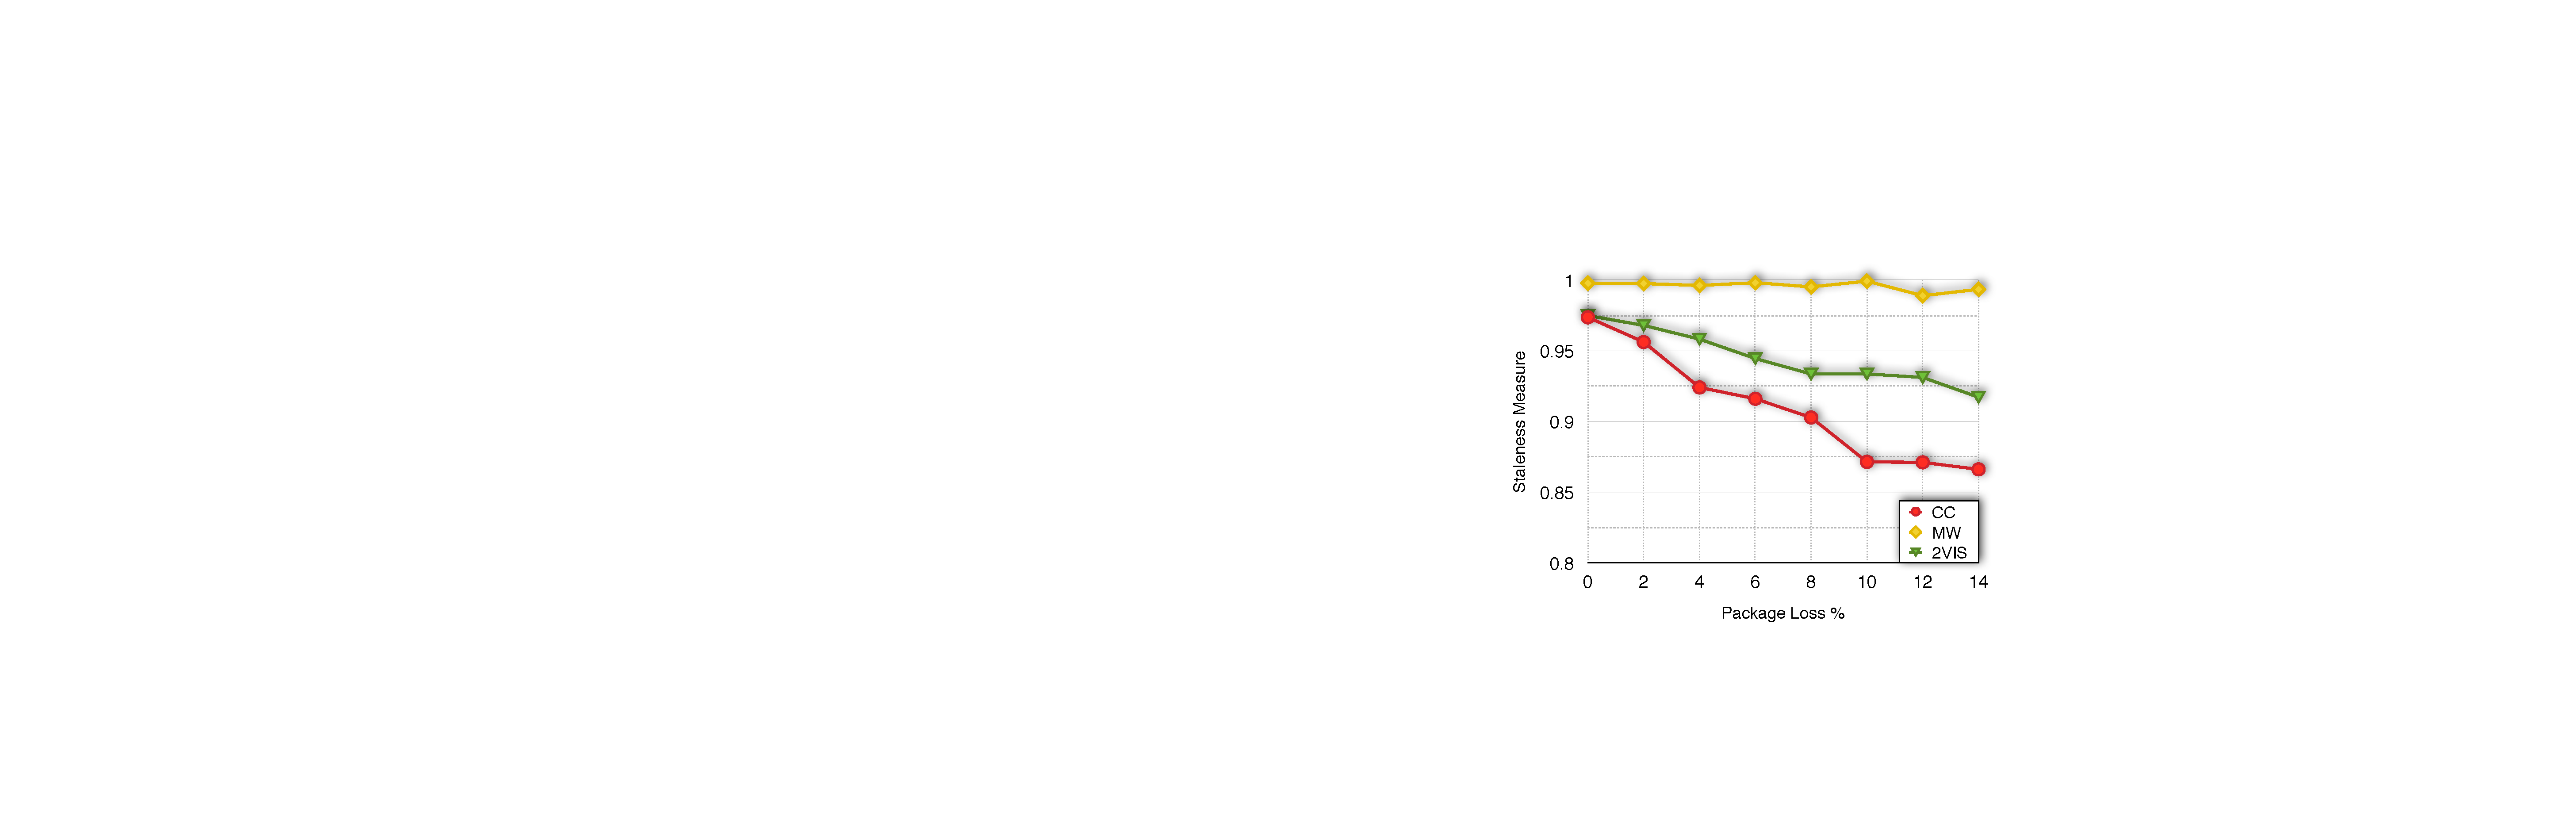
\includegraphics[scale=0.22]{Figures/staleness.pdf}
	\subcaption*{ \hspace{-1mm} (b) Staleness}
	\label{subfig:comment_example}
	\end{subfigure} 
	\begin{subfigure}[t]{0.28\textwidth}
	\centering
	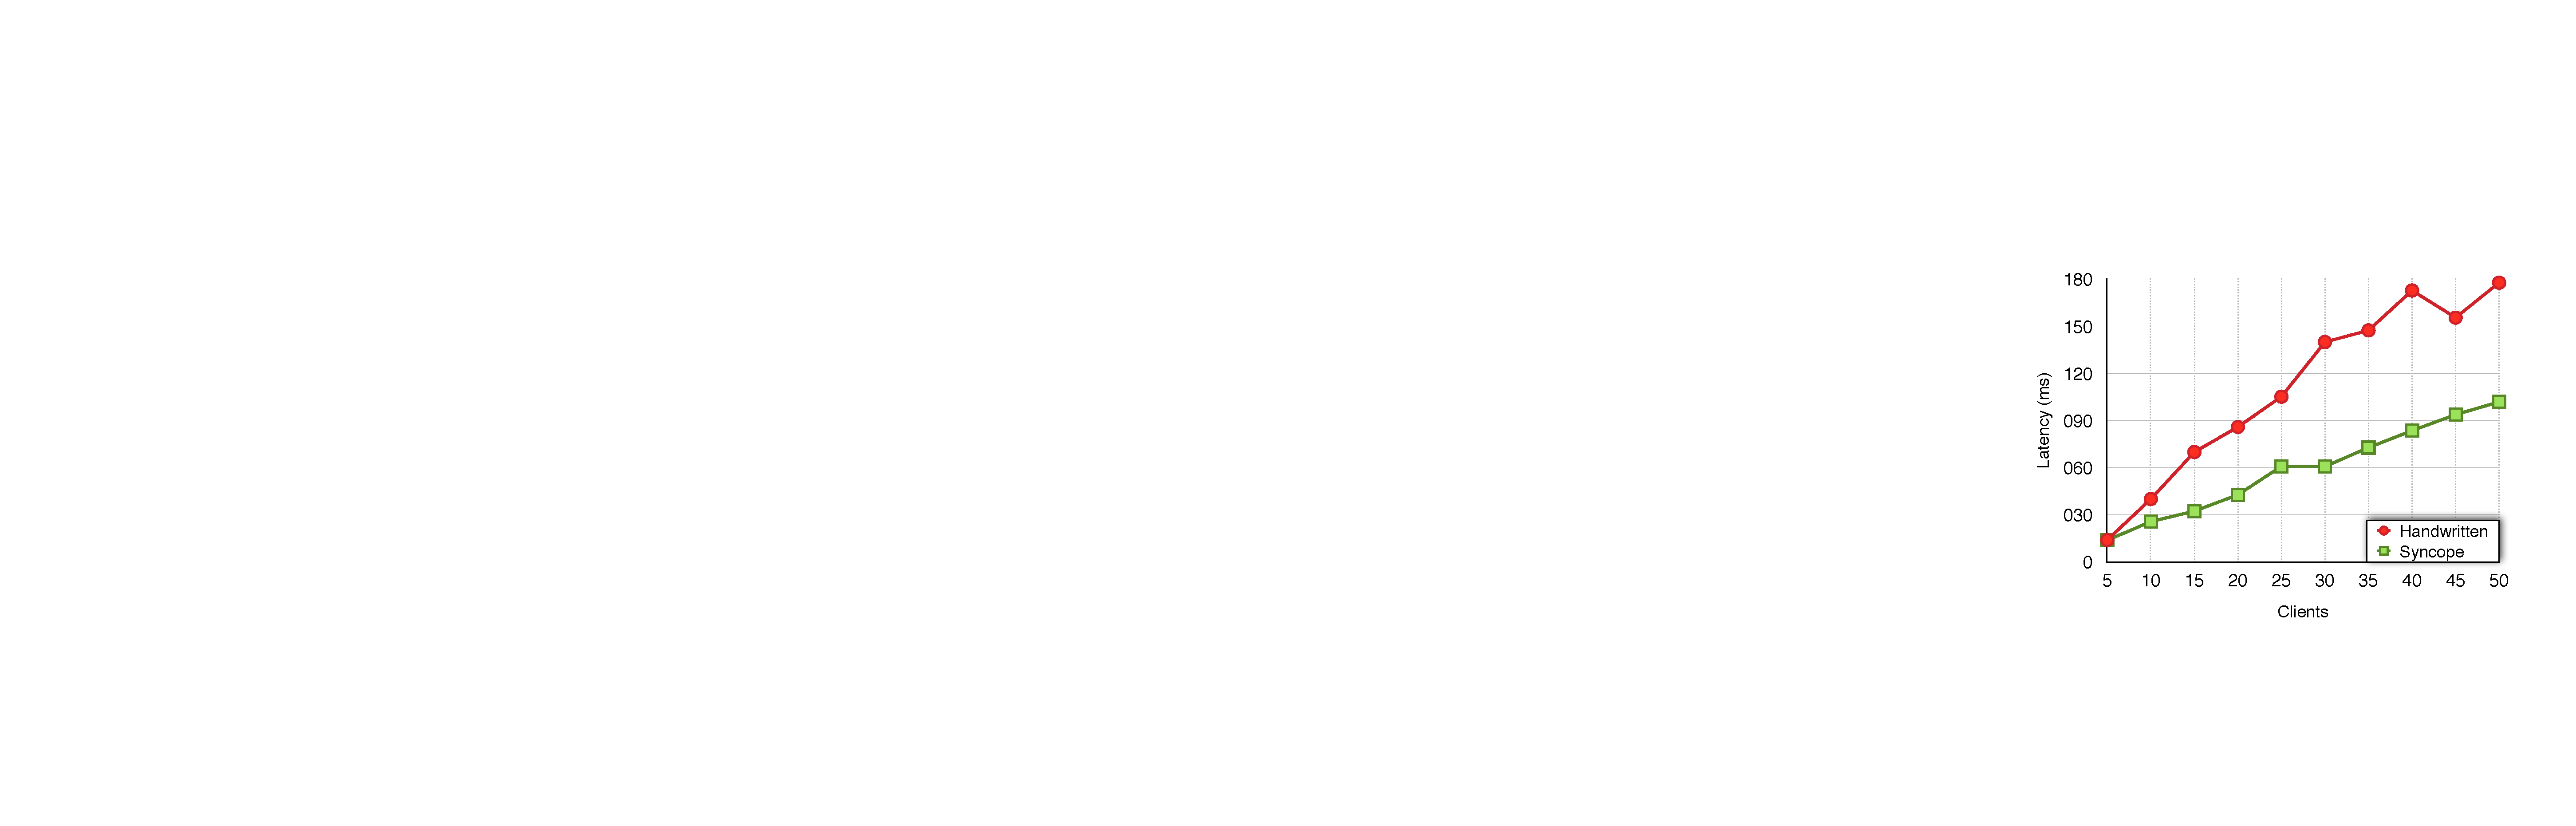
\includegraphics[scale=0.22]{Figures/comparison.pdf}
	\subcaption*{ \hspace{8mm} (c) Manual RMW}
	\label{subfig:comment_example}
	\end{subfigure} 
\\ \hrulefill
\caption{A distributed application for comment section
management}
\label{fig:eval}
\end{figure}



% performance evaluation
For our performance evaluation, we deploy \tool on a cloud cluster,
consisting of three fully replicated Cassandra replicas, running on
seperate machines within the same
datacenter. 
Each machine is instantiated with a
\tool shim layer, that responds to clients,  
 which are instantiated on a VM 
co-located with one of the replicas on a machine.
We deploy the cluster on three \texttt{m4.4xlarge} Amazon EC2 instances
in US-West (Oregon) region, with inter-machine communication delay of 5ms.

% The problem with Cassandra
% ! 
% !
% PLEASE ADD CITATIONS/EDIT -- I WILL BE LOOKING FOR CITATIONS
Inter-replica communications in Cassandra are over TCP connections, 
causing all messages get delivered with no loss and reordering, which
is in practice, far  more consistent than EC, masking out the
performance gain from our fine-grained consistency guarantees.
Consequently, to simulate a
realistic EC environment, we injected artificial message losses at
\tool's shim layer, forcing random messages to be delayed for 1s,
simulating messages losses in a network with roughly 400ms RTT.

%The latency and staleness gain using fine-grained consistency
Fig.~\ref{fig:eval}(a) and \ref{fig:eval}(b) represent
our experimental results, with a workload generated 
by 50 concurrent clients repeatedly running sessions, each composed of three
operations, where operations uniformly choose from 5 objects and are
performed under the specified consistency level. 
We increase the
percentage of delayed messages from 0 to 14, where each experiment ran 
until all clients repeated their session 100 times. Additional to client perceived
latency, we also measure the staleness of operations, which we define as
the average ratio of the number of visible effects,
to the number of all available effects, when executing an operation.

% latency result
In the first set of experiments, we measure latency under
three different \LB{} contracts, all implemented in \tool. As
expected,
causal consistency and RMW experience respectively the highest and the
lowest
performance loss as the percentage of lost messages is increased\footnote{In fact, 
they define the storngest and the weakest
\LB{} dependency relations expressable in our language:
$(\xrightarrow{\soZ})$ and $(\xrightarrow{(\soZ\cup\visZ)^*})$}.
At only $4$ percent message loss rate, we see $17\%$ higher latency under MR
contract compared to RMW, and  $67\%$ higher latency in CC
compared to MR, whereas with $10$ percent message loss, the numbers are
increased to $18\%$ and $87\%$.


%latency result
Similarly, we repeated the experiment with 3 \UB{} contracts, where
\emph{causal visibility} (CV) contract (i.e. {\footnotesize $ \forall a.
a\xrightarrow{(\soZ\cup\visZ)^*;\visZ}\hat{\eta}\Rightarrow a\xrightarrow{\visZ}
\hat{\eta} $}), offers the most stale data when the percentage of lost
messages is increased, whereas staleness in MW is the lowest and is
barely effected. We report $3\%$ ($6\%$) difference 
between staleness of data under MW and 2VIS, and $4\%$ ($7\%$)
difference between 2VIS and CV,
at four (ten) percante message
loss rate.



%handwritten compared
Finally, in order to evidence the practicality of \tool, we implemented
an ad-hoc mechanism to prevent lost-updates anomaly, for a simple
counter application working directly on top of Cassandra. Fig.~\ref{fig:eval}(c) shows the latency results of
this application compared to the \rmwCTRT{} guarantee in \tool, where we report $78\%$
higher latency for the handwritten code compared to \tool with 50
concurrent clients.
Additionally, we experienced many complications with beekkeeping in the handwritten
implementation, mainly because of the lack of meta-data queries in
Cassandra, which forced us to implement a global lock for strongly
consistent table alterations at 
the beginning and the end of each session, as mentioned before.










































